% \begin{tikzpicture}[font=\footnotesize]
% 	\draw (0,-1.5)rectangle(4.5,1.5);
% 	\draw (3,-1.5)--++(0,3);
% 	\draw (3,0)-|(1,1.5);
% 	\pile{}{12\,V};
% 	\pile{shift={(4.5,0)}}{6\,V};
% 	\resistanceV{shift={(3,0.75)}}{};
% 	\resistanceV{shift={(3,-0.75)}}{};
% 	\resistanceH{shift={(2,1.5)}}{};
% 	\resistanceH{shift={(2,0)}}{};
% 	\draw[->,shift={(3.25,.75)}](0,-.5)--++(0,1)node[midway,right]{$U_1$};
% 	\draw[->,shift={(2,1.75)}](-0.5,0)--++(1,0)node[midway,above]{$U_2$};
% 	\draw[->,shift={(2,-.25)}](0.5,0)--++(-1,0)node[midway,below]{$U_3$};
% 	\draw[->,shift={(3.25,-.75)}](0,-0.5)--++(0,1)node[midway,right]{5\,V};
% \end{tikzpicture}
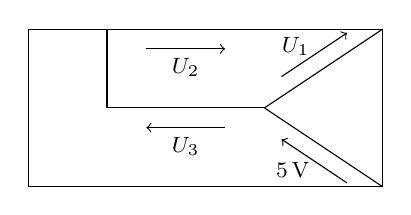
\begin{tikzpicture}[font=\footnotesize]
	\draw (0,-1)rectangle(4.5,1);
	\draw (4.5,1)--(3,0)--(4.5,-1);
	\draw (3,0)-|(1,1);
	\FEMVL{}{12\,V};
	\FEMVR{shift={(4.5,0)}}{6\,V};
%	\pileL{}{12\,V};
%	\pileR{shift={(4.5,0)}}{6\,V};
	\resistanceH{shift={(3.75,0.5)},rotate=33.7}{};
	\resistanceH{shift={(3.75,-0.5)},rotate=-33.7}{};
	\resistanceH{shift={(2,1)}}{};
	\resistanceH{shift={(2,0)}}{};
	\draw[->,shift={(3.75,.5)},rotate=33.7](-.5,6pt)--++(1,0)node[pos=.7,left=3pt]{$U_1$};
	\draw[->,shift={(2,0.75)}](-0.5,0)--++(1,0)node[midway,below]{$U_2$};
	\draw[->,shift={(2,-.25)}](0.5,0)--++(-1,0)node[midway,below]{$U_3$};
	\draw[->,shift={(3.75,-.5)},rotate=-33.7](0.5,-6pt)--++(-1,0)node[pos=.3,left=3pt]{5\,V};
\end{tikzpicture}